%% LyX 2.0.2 created this file.  For more info, see http://www.lyx.org/.
%% Do not edit unless you really know what you are doing.
\documentclass[english]{article}
\usepackage[T1]{fontenc}
\usepackage[latin9]{inputenc}
\usepackage{listings}
\usepackage{geometry}
\geometry{verbose,tmargin=2.2cm,bmargin=3cm,lmargin=1.6cm,rmargin=1.6cm}
\usepackage{url}
\usepackage[pdftex]{graphicx}
\usepackage{capt-of}

\lstset{
	basicstyle=\small
}

\makeatletter
%%%%%%%%%%%%%%%%%%%%%%%%%%%%%% User specified LaTeX commands.
\usepackage{babel}






\usepackage{babel}




\usepackage{babel}

\makeatother

\usepackage{babel}
\begin{document}

\title{Software Engineering Coursework 2}


\author{Abhijit Chandgadkar, Osama Javed, Joseph Slade, Cliff Sun, Luke Tomlin}


\date{06/12/12}

\maketitle

\section*{Process}

Acting as a small team tackling a completely unfamiliar codebase,
we took several steps towards implementing the desired goal, keeping
in mind extra aims to improve the existing code, make it maintainable
and make it extendable.


\subsection*{Adding unit tests for existing functionality}


\paragraph*{What}

Whilst we had many ideas for improving the code itself, the most important
part was to make sure that we did not affect the existing functionality
beyond what we were asked to change, effectively 'freezing' the current
functionality. To do this, we began adding unit tests that tested
the existing functionality, so that we could easily verify that our
changes were not breaking anything. This was the first step to making
the code maintainable, much like we did in the first lecture tutorial
(Legacy Code). We decided to use $JUnit4$ to do our unit testing,
with some help from $JMock$.


\paragraph*{How}

We had aspirations to restructure the project to make it more easily
maintainable - this meant that we had to add tests for all of the
areas that we were planning to touch. As an example, the project specification
had us editing the $BillingSystem$ class. Upon inspection, we decided
what responsibilities this class had: 
\begin{itemize}
\item Registers calls starting and ending between numbers 
\item Processes these calls and applies them as bills to the corresponding
customers from the customer database

\begin{itemize}
\item In doing so, it reads the tariff rates and uses them with some algorithm
(which we were changing in the specification) to decide the final
cost of the call. 
\end{itemize}
\end{itemize}
Judging from these responsibilities, we added a variety of unit tests
covering basic and edge cases for each responsibility. For instance,
for $callInitiated$ and $callCompleted$, we added tests to make
sure that the specified events were added to the log.

We realised that writing a unit test for $createCustomerBills$ would be
highly cumbersome as it was calling $createBillFor$ for every customer.
The entire telephony logic of the system resided in this function. 

After thoroughly reading and understanding the algorithm, we carefully extracted some of the logic out into separate private functions. Although this was not necessary but it significantly improved the readability of the algorithm and also allowed us to scrutinise the different responsibilities inside the logic. After this, we carefully started refactoring the different parts of the logic into new classes. This allowed us to write tests for each aspect of the logic separately and thus we eventually finished testing out the entire billing algorithm. For example one part of the logic which we refactored was where the call time was being checked to see whether it lied between the peak period using $DaytimePeakPeriod$ and then calculated the cost of the call accordingly. We split this functionality out into two interfaces, $TimeCalculator$ and $CallCostCalculator$. We also introduced $PeakOffPeakTime$ with the sole purpose of storing a value for peak time and off-peak time.

\begin{lstlisting}[language=Java]
public interface TimeCalculator{
PeakOffPeakTime calculateTimes(long startTime, long endTime);
}

public interface CallCostCalculator {
BigDecimal calculateCost(final PeakOffPeakTime peakOffPeakTime,
final Tariff tariff);
}

public class PeakOffPeakTime{
private final long peakTime;
private final long offPeakTime;
}

.
..
PeakOffPeakTime peakOffPeakTime = timeCalculator.calculateTimes(call.getStartTime(), call.getEndTime());
BigDecimal callCost = callCostCalculator. calculateCost(peakOffPeakTime, tariff);
..
.

\end{lstlisting}

The implementation for $TimeCalculator$ would contain $DaytimePeakPeriod$ which would be used to calculate and return the total number of time the call was in the peak period and off-peak period. In the case of the original algorithm, one of these values would be 0 because if a call overlapped on to a peak period the whole call was treated as peak call. The implementation of $CallCostCalculator$
would then return the cost of the call given the peak and off-peak duration. The advantage of this refactoring step was twofold. One it allowed us to easily write unit tests for each aspect of the logic, i.e. it became much simpler to think of test cases and also to write them instantly. Having tested legacy code gave us enough confidence to make further refactoring including making use of DateTime and optimising the current solution. Secondly it allowed us to efficiently split the work between our team members. For example, a new implementation of $TimeCalculator$ was being developed concurrently which would calculate the total peak and off-peak time in a call based on the new requirements. This would then be passed on to $CallCostCalculator$ to calculate the cost of the call based on the tariff. 

We previously had not planned on using interfaces but our design evolved as we started writing unit tests. This was because we were using mocks as we didn't want to test every part of the logic functionally. In many places we simply wanted to see whether the correct classes were making the correct function calls with the correct parameters. An example code-snippet of a test for $TimeCalculator$ was as follows:

\begin{lstlisting}[language=Java]
context.checking(new Expectations(){{
oneOf(timeCalculator).calculateTimes(startTime, endTime); will(returnValue(peakOffPeakTime));
oneOf(callCostCalculator).calculateCost(peakOffPeakTime, tariff); will(returnValue(callCost));
oneOf(lineItemFactory).createCallLineItem(call, "callee", callCost, peakOffPeakTime); will(returnValue(lineItem));
}});
new DefaultTotalBillCalculator(callCostCalculator, lineItemFactory, timeCalculator).calculateTotalBill(calls, tariff, lineItems);
\end{lstlisting}

Nevertheless, for testing $CallCostCalculator$, we didn't feel it was necessary to use mocks as we simply wanted to see whether it correctly returned the expected result.

\begin{lstlisting}[language=Java]
public void testCallCostWithStandardTariff() throws Exception {
PeakOffPeakTime peakOffPeakTime = new PeakOffPeakTime(100, 200);
    Tariff tariff = Tariff.Standard;
    BigDecimal cost = new DefaultCallCostCalculator().calculateCost(peakOffPeakTime, tariff);
    Assert.assertEquals(cost.longValue(), 90);
 } 
\end{lstlisting}

While making these modifications, an important consideration other than preserving original behaviour was to not modify the public interface of $BillingSystem$. We ensured that the signature of the public methods remained the same and that no new exceptions were thrown. This was because all the clients that use of our jars would then have to modify the way they would be calling our billing system as otherwise their system would break. In real life, if there were were several users using our classes, it would be very expensive to make such changes. However in order to test our billing system, we overloaded the constructor to take in the necessary parameters and also created a function $fullCompletedCall$ to avoid having to use $Thread.sleep$ in our tests.


\subsection*{Forming specifications for new functionality}

In our project with Stephen, our entire project goals had been specified
by mouth only! As we saw in week 5 of the lecture (Spec by Example),
this is quite risky - we might completely misinterpret what Stephen
meant, and end up wasting time in the process. To remedy this, we
decided to create a simple DSL using JUnit, with which we created
some acceptance tests. This meant that the tests were easily readable,
simple to write, and were simple to demonstrate to Stephen and other
non-developers as an example of expected operation. The results of
these tests could also be printed as a normal bill.


\paragraph*{Acceptance tests}

Writing acceptance tests is crucial for both development and the business.
For developers it provides validation that a particular feature works
across the whole system. Acceptance tests tells the business that the feature
has been successfully implemented and can be released to production.
In our case, it is important to write acceptance tests for the new
functionality that we are required to implement, as it allows our customer
Stephen to see whether new functionality works and also lets him know
how development is progressing . In addition, as we aimed to refactor the existing 
codebase to bring it out of legacy (to allow testing to be easily done), it is 
necessary for us to write acceptance tests for the old functionality. This way we 
can validate that the existing functionality is still working. 

\paragraph*{How}

Using parts of week 6's lectures (DSLs), we developed our own DSL
to perform the acceptance tests. Below is an example of one of the
tests

\begin{lstlisting}[language=Java,showstringspaces=false]
// Creating a new customer database
customerDatabase = createNewDatabaseWithCustomers(
	aCustomer(named("James"),  	
		  withTelephoneNumber("+447567891234"),  					   				 
		  withTariffPlan("Standard")), 					   						  
	aCustomer(named("Fred"),  					   							
		  withTelephoneNumber("+447912345678"),  					   			
  		  withTariffPlan("Standard"))
);

// Testing the final bill printed
givenAcmeTelecom().hasCustomerDatabase(customerDatabase).
	andHasABillingSystem(
	billingSystem().withTelephoneCalls(telephoneCalls).
			withABillPrinter(billPrinter)
	weExpectTheFollowingBillToBePrinted(
		aBill(forCustomer(customer(named("James"), customerDatabase), 
				  usingPrinter(aStandardPrinter())).
		      withACall(startTime(telephoneCall1StartTime),
				endTime(telephoneCall1EndTime),
				toReceiver(customer(named("Fred"), customerDatabase)),
				withCost("7.20")).
		      withBillTotal("7.20"),
		      //another bill for Fred )).
	assertResultWith(billPrinter);
	
\end{lstlisting}
The benefits of such an acceptance test system are immediately obvious
- it lets someone without any prior knowledge of how Java works or
of how the system is set up, understand what the tests are doing -
a developer could run through this code with Stephen or any other
project manager, and change the acceptance tests (and ultimately the
code itself to adhere to the tests). This was built up using a combination
of builder patterns (for building the tests from the DSL), fixtures
(for running the tests), and microtypes (to make the DSL more readable). 


\paragraph*{Choice}

We can choose a variety of acceptance test frameworks to write out
tests with. Frameworks like Behave, FIT and Cucumber are well supported
and widely used but often come with a lot of setting up and have features
that are not necessary in our case as we only needed to
test that we charge the correct amount depending on the peak period.
So in our case it would be beneficial to write out own DSL to create
acceptance tests with. The advantage is that we can write out DSL in the host 
language and allows us to use a well-known and widely used framework 
to write our acceptance test (JUnit). Also, as we are doing this in an IDE,
we have the advantages of auto-complete, content assist and syntax
checking. 

\subsection*{Adding unit tests for new functionality}

Before we could implement the required changes, we wanted to add unit
tests to cover what the expected outcome was going to be, as an example
of Test-Driven Development. This meant that we could repeatedly test
the code as we implemented it to ensure that the desired goal was
being fulfilled. In addition writing unit tests before implementing the actual
code helped us to drive the design of our code and as a result we ended 
up with much more modular design. We also had to think carefully about 
what exactly to test, to make sure that it completely covered every aspect 
of our goals.

\begin{lstlisting}[language=Java]
@Test     
public void testCallCostWithStandardTariff() throws Exception {     	
	PeakOffPeakTime peakOffPeakTime = new PeakOffPeakTime(100, 200);     	
	Tariff tariff = Tariff.Standard;     	
	BigDecimal cost = 
		 new DefaultCallCostCalculator().calculateCost(peakOffPeakTime, tariff); 
	Assert.assertEquals(cost.longValue(), 90);     
}	
\end{lstlisting}

\subsection*{Implementing new functionality}

By this point we were fairly confident that we had a good grasp of
the existing functionality that we needed to preserve, cemented by
unit tests, as well as a good vision of what we needed to add/change,
supported by the acceptance tests written in the DSL (which we would have
cleared with Stephen).

We decided to use a test-driven approach to implement the required changes.
This meant that we could repeatedly test the code as we implemented it to ensure 
that the desired goal was being fulfilled. In addition writing unit tests first helped us to drive the
design of our code and as a result produce a modular
design. 


\paragraph*{What}

The task of adding the new functionality was twofold. One to develop an algorithm to
calculate the peak and off-peak time given the start time and the end time of a call. Secondly clients should easily be allowed to read and specify the peak time periods.


OSAMA CAN TALK ABOUT THIS

We needed to tweak how the calls were charged, which involved understanding
exactly how long a call was in peak and offpeak periods and tallying
the results accordingly. This involved recoding how $BillingSystem$
worked, as well as moving and/or adding functionality to $DaytimePeakPeriod$.


\paragraph*{How}

We created a new package called timeutils, which abstracted the required
peak/offpeak time calculations out from the billing system. Careful
consideration went into building the package, making sure that it
would be easily scalable and configurable. For instance, we added
the ability to define different xml files for peak/offpeak configuration,
which are read in at run-time, and they also allow multiple peak and
offpeak times to be specified for the same day.

Originally we considered making the time calculation methods static,
to improve performance - however after rethinking the issue we decided
to use interfaces and objects as this is much easier to scale and
extend. If the underlying implementation needs to change at any point
(eg. implementing a different kind of calculator), as long as they
abide by the interface rules everything will still work. 

This package was developed in a test-driven-development style - unit
tests were specified once the planning had finished, and were coded
to cover the entire scope of the specification. The result of this
was that we could be confident that the required functionality was
intact as we went about developing the package.

The end result was a change in how $BillingSystem$ worked, as well
as removing a lot of the responsibility that it previously had. It
fundamentally performed the same task, however it now did so more
efficiently, and in a much clearer and concise manner.


\subsection*{Refactoring and improving code to aid maintainability and code health}

The existing code had multiple problems that we aimed to fix over
the course of the project. These were not all related to the goals
set out by Stephen, but as we would be looking after the codebase
for the forseeable future we decided that it would be wise to improve
the general health of the codebase to reduce headaches later. Some
examples: 
\begin{itemize}
\item The $DaytimePeakPeriod$ class, which handled deciding whether calls
were onpeak or offpeak, was very rigidly implemented. The times for
the boundary between offpeak and peak were defined as ``magic numbers''
inside the code (in this case as 7 and 19, representing 7am and 7pm
respectively). This left no room for providing flexible peak and offpeak
times without directly editing the class itself. Additionally, if
different tariffs could have different peak times, perhaps changing
more than once throughout the day, it would require a whole overhaul
of the class. 
\item The $CallStart$ and $CallEnd$ classes, used $System.currentTimeMillis$
to get the time of call and end. This made testing difficult - to
construct a call using this implementation would require the test
to $sleep$ inbetween calling and ending the call, which would make
the testing process very slow indeed! This occurs in the $Runner$
example provided in the specification - it takes a full 1 minute and
50 seconds to complete!
\item The $BillingSystem$ was responsible for registering and handling
$CallEvent$ happenings, which we felt was somewhat outside of its
domain of responsibility. We felt that a system that is designed for
billing should handle just that - it should take a list of pre-assembled
calls, and work out the bills from that. 
\item Additionally, the $BillingSystem$ was woefully inefficient at creating
the bills for customers. In the original state, it would iterate through
every customer, and then through every $CallEvent$ that had been
logged, and assemble each call that way. If, for example, the system had $1000$
customers, and each customer makes $100$ calls over the course of
the month, then each customer adds $200$ different events to
the $callLog$, for a total of $200,000$ call events. That means that
the $BillingSystem$ makes a total of $1,000\, customers\times200,000\, events=200,000,000$
iterations to assemble one bill for all of its customers! Even generating
a single bill takes $20000$ iterations, making this system very difficult
to scale. This isn't even the worst case - the way the system is designed,
it searches the whole $callLog$ every time!
\end{itemize}

\paragraph*{How}

We performed many different changes to the code, with the aim to fix
the above problems, or at least make them more manageable. Some of
the main things we changed include:


\subparagraph*{Call Events}

We added an $AbstractCallEvent$ as an abstract interface implementing
the $CallEvent$ interface, and then changed $CallStart$ and $CallEnd$
to implement this. This let us write tests a lot more easily (rather than
having to rely on $sleep$!), by letting us fabricate times as we
wanted and then test it using the standard functions. Additionally,
we implemented the common $getCaller$ and $getCallee$ methods that
were being duplicated in both $CallStart$ and $CallEnd$ inside the
$AbstractCallEvent$ class, reducing the code size and making it easier
to read. As an example, this reduced the $CallStart$ class to simply
being

\begin{lstlisting}[language=Java]
public class CallEnd extends AbstractCallEvent {
	public CallEnd(String caller, String callee) {
		super(caller, callee, System.currentTimeMillis());
	}
}
\end{lstlisting}



\subparagraph*{BillingSystem}

With the $BillingSystem$ class, we made a lot of changes. From the
performance perspective, we moved the calculation of bills from call
events to happen as the calls come in - this made it far more efficient
when bill generation was required, effectively making it linear in
size of customer base as compared to quadratic! From the structure
perspective, as mentioned above, we moved a lot of the functionality
elsewhere and made its responsibilities more specific. Additionally,
we added a large amount of extra functionality to the existing system,
such as allowing for flexible peak/offpeak time periods, or even multiple
peak/offpeak time periods! These can be defined at run-time using
xml, and were implemented using the $JAXB$ java architecture for
xml bindings. Basic validation of these files is done at runtime to
ensure that they are properly formed, and helps prevent user-created
errors.


\subparagraph*{Joda Time}

One big change that we made to the code was to introduce Joda Time
(\url{http://joda-time.sourceforge.net/}) in place of $java.util.Date$.
This had many advantages, above and beyond simply being easier to
use. It has a lot more flexibilty and power than $Date,$ allowing
us to work dates and times in a more concise manner without having
to wrestle with $Calendars$ and $SimpleDateFormat$ classes. Another
big thing to consider was the fact that $SimpleDateFormat$ is not
thread safe! As handling dates and times is so integral to the code,
if we wanted to implement any sort of multi-threading functionality
to the code we would have to completely remove $SimpleDateFormat$. 


\section*{Class and Package Hierarchy}

The initial source code we received had all the classes in one package. This makes our package very cohesive and hard to maintain as all the responsibility lies in one single package. In our refactoring process we started to move responsibilities out into separate packages. This was aided by our test driven design process which promoted a more modular package and class design. In figure 1 you can see that the class dependency structure is quite cohesive, BillingSystem and BillGenerator are quite coupled and there are cyclic dependencies between them.
After refactoring you can see that 

\begin{center}
  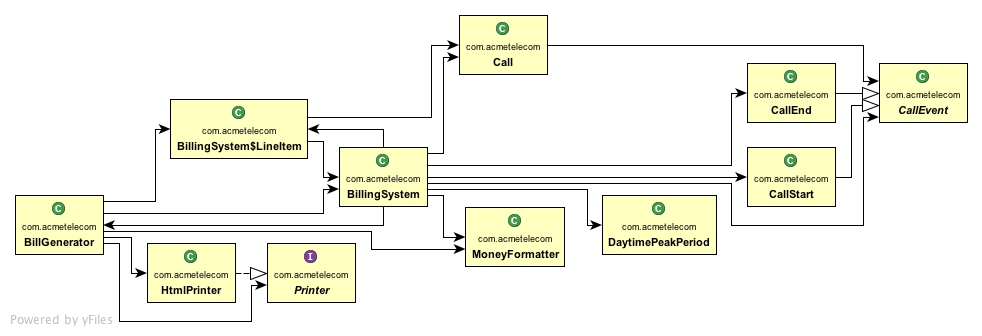
\includegraphics[scale=0.41]{initialclassdependencies.png}
  \captionof{figure}{Class Dependencies For Initial Source Code}
  \label{fig:initialclassdependencies}
\end{center}



\begin{center}
  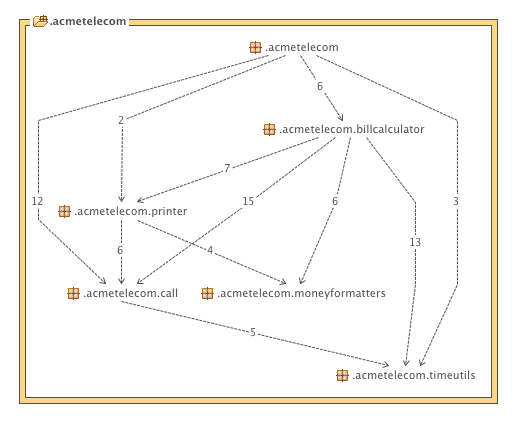
\includegraphics[scale=0.46]{moduledependencies.png}
  \captionof{figure}{Class Dependencies For Initial Source Code}
  \label{fig:initialclassdependencies}
\end{center}

\section*{Considerations}

Whilst we were implementing the required changes and tweaking the
codebase, we thought of a variety of other considerations that should
be considered. We also implemented some of these whilst we were coding,
but some of the other ones were outside the scope of the coursework
itself, but should have been considered in the theoretical Acme Telecom
scenario.


\subsection*{Source control}

When we first received the code from Stephen, it was simply emailed
as a tarball. Keeping the code like this was definitely sub-optimal,
so we decided to host it in some form of source control (in our project
we used GitHub for ease of use - but in the context of Acme Telecom
we would most likely have used a private version!). This made collaboration
between the team members much easier, as well as keeping a timeline
of changes made to allow rollbacks.


\subsection*{Architecture changes}

We made multiple architectural changes to the code over the course
of the project - we altered where some of the files were placed, based
on responsibilities, as well as adding testing (acceptance or unit-based)
and resource directories. For instance, we moved calling-based and
call-event-based classes away from normal telecom-based classes into
a seperate package, moved the entirety of offpeak/peak cal calculations
out to a seperate utils class, amongst other things, modularising
the codebase and making it easier for multiple people to work on different
areas of the program, as well as making the code conceptually easier
to understand. 


\paragraph*{Wrappers}

We found that testing was a little bit challenging, as the customer
database that was supplied to us was located outside of the package.
We considered creating a wrapper around the functionality of the database,
which we could use as an interface to create dummies of the database
for testing and mocking without having to touch the 'real' databases
whilst doing tests. However, we didn't have enough time to fully implement
these wrappers. Fortunately this doesn't translate too badly into real
life, as the database accesses that are performed from the tests are
minor, but this could be problematic if the databases are ever down
and we need to do tests!


\subsection*{Multi-Threading}

The act of generating multiple bills appears to lend itself quite
well to a multi-threaded approach. Each bill being generated could
be classified as a unit of operation, and the whole process could
be split across multiple computers. We did not get around to implementing
multithreading to the system, but it would certainly be something
to consider in the future if running time ever became a problem. 


\subsection*{Licensing}

Some care needed to be used when thinking about what OpenSource software
we wanted to use. If any of these had a 'viral' license (such as the
GNU General Public License), which require all derivative works to
also be licensed with the GPL, then the whole project itself would
have to be licensed with the GPL! This might prove to be problematic
in a private company with proprietary software, as they most likely
do not want competitors to be able to freely use their software. However,
because we would not have been distributing the binaries for the billing system,
this would not have been an issue. We had to consider this risk when
 deciding to use Joda Time, for instance.
Fortunately, Joda Time uses the Apache 2 license, which is not 'viral'
and only requires that derivative work contains notifications of what
was changed, as well as retaining all other copyright, patent, trademark
notices etc. that existed in the original.

Maven also helps us with licensing - it can keep track of license
for different parts of the projects, and notify us of clashes in licensing. 


\subsection*{Building}

For build automation we decided to use Maven, as the team was already
mostly familiar with its usage from previous tutorials, and because
of how well it tied in with TeamCity for continuous integration.
Additionally, it allowed the import of our project as a dependency,
so it could be easily used in other projects (such as extensions of
the billing system or similar).


\subsection*{Deployment}

Whilst we did not actually implement any deployment mechanisms, we
did consider what deployment mechanisms would be appropriate for Acme
Telecom in the case of this product. Given the suite of tests that
we created testing for both the new and the old functionality, and
our use of Maven and git for source control and building, we thought
that it would be best to use TeamCity, much like we did in week 7's
tutorial (Release). It would be fairly simple to set up as we already
had git and Maven configured, and assuming that management was happy
with the quality of the tests that we put in place, would make releasing
very simple and quick. We assumed that the Acme company has access
to its own set of servers, and we would use those to deploy on.

However, 'pushing to production' would not probably not be a suitable
 model for the billing system of a telecom company. An error in billing
would almost always lead to big issues for the company, either costing
them money, reputation or both.

Maven also acts as a form of internal deployment - it lets us deploy
to an internal 'Maven repository'. Internal users who wish to use
the latest version of our project simply add the project as a dependency
to their project, and Maven then automatically imports the latest
version of the jars and sets it up.
\end{document}
